\let\negmedspace\undefined
\let\negthickspace\undefined
\documentclass[journal]{IEEEtran}
\usepackage[a5paper, margin=10mm, onecolumn]{geometry}
\usepackage{tfrupee} % Include tfrupee package

\setlength{\headheight}{1cm} 
\setlength{\headsep}{0mm}     

\usepackage{gvv-book}
\usepackage{gvv}
\usepackage{cite}
\usepackage{amsmath,amssymb,amsfonts,amsthm}
\usepackage{algorithmic}
\usepackage{graphicx}
\usepackage{textcomp}
\usepackage{xcolor}
\usepackage{txfonts}
\usepackage{listings}
\usepackage{enumitem}
\usepackage{mathtools}
\usepackage{gensymb}
\usepackage{comment}
\usepackage[breaklinks=true]{hyperref}
\usepackage{tkz-euclide} 
\usepackage{listings}
\def\inputGnumericTable{}                                 
\usepackage[latin1]{inputenc}                                
\usepackage{color}                                            
\usepackage{array}                                            
\usepackage{longtable}                                       
\usepackage{calc}                                             
\usepackage{multirow}                                         
\usepackage{hhline}                                           
\usepackage{ifthen}                                           
\usepackage{lscape}
\usepackage{circuitikz}
\tikzstyle{block} = [rectangle, draw, fill=blue!20, 
    text width=4em, text centered, rounded corners, minimum height=3em]
\tikzstyle{sum} = [draw, fill=blue!10, circle, minimum size=1cm, node distance=1.5cm]
\tikzstyle{input} = [coordinate]
\tikzstyle{output} = [coordinate]


\begin{document}

\bibliographystyle{IEEEtran}
\vspace{3cm}

\title{4.13.1}
\author{AI25BTECH11036-SNEHAMRUDULA}
 \maketitle
{\let\newpage\relax\maketitle}
\renewcommand{\thefigure}{\theenumi}
\renewcommand{\thetable}{\theenumi}
\setlength{\intextsep}{10pt} 
\numberwithin{equation}{enumi}
\numberwithin{figure}{enumi}
\renewcommand{\thetable}{\theenumi}
\textbf{Question}:\\
\textbf{Q.}\;
\begin{question}
\begin{question}
Consider the lines given by
\begin{align*}
L_1 &: x + 3y - 5 = 0, \\
L_2 &: 3x - ky - 1 = 0, \\
L_3 &: 5x + 2y - 12 = 0.
\end{align*}
Match the Statements/Expressions in Column I with the Statements/Expressions in Column II.

\begin{center}
\begin{tabular}{p{0.45\linewidth} p{0.45\linewidth}}
\textbf{Column I} & \textbf{Column II} \\
\begin{enumerate}[label=(\Alph*)]
    \item $L_1, L_2, L_3$ are concurrent, if
    \item One of $L_1, L_2, L_3$ is parallel to at least one of the other two, if
    \item $L_1, L_2, L_3$ form a triangle, if
    \item $L_1, L_2, L_3$ do not form a triangle, if
\end{enumerate}
&
\begin{enumerate}[label=(\alph*)]
    \item $k = 9$
    \item $k = \dfrac{-6}{5}$
    \item $k = \dfrac{5}{6}$
    \item $k = 5$
\end{enumerate}
\end{tabular}
\end{center}
\end{question}
  
\\ 
\solution \\
\begin{solution}
The general form of a line is $\vec{n}^\top \vec{x} = p$, where $\vec{n}$ is the normal vector.

For the given lines:

\begin{align*}
L_1 &: \vec{n}_1 = \begin{pmatrix} 1 \\ 3 \end{pmatrix}, \quad p_1 = 5, \\
L_2 &: \vec{n}_2 = \begin{pmatrix} 3 \\ -k \end{pmatrix}, \quad p_2 = 1, \\
L_3 &: \vec{n}_3 = \begin{pmatrix} 5 \\ 2 \end{pmatrix}, \quad p_3 = 12.
\end{align*}

\begin{enumerate}[label=(\Alph*)]
    \item \textbf{Concurrent:} The lines are concurrent if the matrix
    $\begin{pmatrix} 1 & 3 & -5 \\ 3 & -k & -1 \\ 5 & 2 & -12 \end{pmatrix}$
    has determinant zero.

    Computing the determinant:
    \begin{align*}
    &1((-k)(-12) - (-1)(2)) - 3(3(-12) - (-1)(5)) + (-5)(3(2) - (-k)(5)) \\
    &= 1(12k + 2) - 3(-36 + 5) - 5(6 + 5k) \\
    &= 12k + 2 + 93 - 30 - 25k \\
    &= -13k + 65.
    \end{align*}
    Setting it equal to zero: $-13k + 65 = 0 \Rightarrow k = 5$.

    So concurrent if $k = 5$. Hence (A) matches with (s).

    \item \textbf{Parallel:} Two lines are parallel if their normal vectors are scalar multiples.

    Checking pairs:

    \begin{itemize}
        \item $\vec{n}_1$ and $\vec{n}_2$: $\frac{3}{1} = \frac{-k}{3} \Rightarrow k = -9$.

        \item $\vec{n}_2$ and $\vec{n}_3$: $\frac{3}{5} = \frac{-k}{2} \Rightarrow k = \frac{-6}{5}$.

        \item $\vec{n}_1$ and $\vec{n}_3$: $\frac{1}{5} = \frac{3}{2}$, which is false ⇒ not parallel.
    \end{itemize}

    So parallel if $k = \frac{-6}{5}$. Hence (B) matches with (q).

    \item \textbf{Form a triangle:} The lines form a triangle if they are neither concurrent nor parallel.

    So $k \neq 5$ and $k \neq \frac{-6}{5}$.

    A typical example is $k = 9$. Hence (C) matches with (p).

    \item \textbf{Do not form a triangle:} The lines do not form a triangle if they are either concurrent or two of them are parallel.

    Hence possible when $k = 5$ or $k = \frac{-6}{5}$.

    Here the option is $k = 5$. Hence (D) matches with (s).
\end{enumerate}
\end{solution}
\begin{figure}[h!]
    \centering
    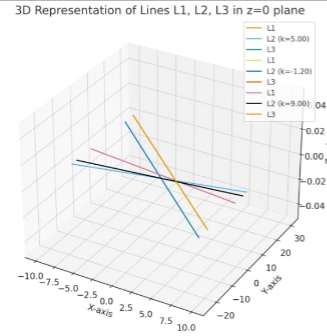
\includegraphics[height=0.5\textheight, keepaspectratio]{fig4.13.1.png}
    \label{figure_1}
\end{figure}
 
\end{document}